\documentclass[reprint,english,notitlepage]{revtex4-2}
\usepackage{amsmath}
\usepackage[mathletters]{ucs}
\usepackage[utf8x]{inputenc}
\usepackage[english]{babel}
\usepackage{esint}
\usepackage{physics,amssymb}
\usepackage{graphicx}
\usepackage{xcolor}
\usepackage{hyperref}
\usepackage{listings}
\usepackage{subfigure}
% \usepackage[style=science, backend=biber]{biblatex}
% \addbibresource{References_Part_4.bib} TODO: Slett før innlevering
\hypersetup{
    colorlinks,
    linkcolor={red!50!black},
    citecolor={blue!50!black},
    urlcolor={blue!80!black}}

\lstset{inputpath=,
    backgroundcolor=\color{white!88!black},
    basicstyle={\ttfamily\scriptsize},
    commentstyle=\color{magenta},
    language=Python,
    morekeywords={True,False},
    tabsize=4,
    stringstyle=\color{green!55!black},
    frame=single,
    keywordstyle=\color{blue},
    showstringspaces=false,
    columns=fullflexible,
    keepspaces=true}

\begin{document}

\title{Landing the rover on the destination planet}
\author{Candidates: 15369 \& 15401}
\date{\today}
\affiliation{Institute of Theoretical Astrophysics, University of Oslo}

\begin{abstract}
    Using a simulation, a procedure for the landing of the lander, and values for the initial position and velocity of the spacecraft have been obtained to land as close to the landing site as possible.
    The lander and parachute were deployed at the same height as in the simulation, but the lander started deviating from the simulated trajectory by descending much slower drifting therefore further east than anticipated.
    This was found to be due to a higher drag force on the lander and parachute during the landing compared to the simulation.
    Nevertheless, the lander was able to execute the landing procedure, and landed 269 meters east from the targeted landing site.
\end{abstract}

\maketitle

\onecolumngrid
\section{Information} \label{sec:info}
\begin{center}
    In this paper we would like to only be graded based on the programming, results and discussion.
\end{center}
\vspace{20}
\twocolumngrid

\section{Results} \label{sec:results}
    To land the rover safely without breaking any parts, the radial velocity towards the planet must not exceed 3 meters per second.
    According to our calculations, this would require a parachute area of 406 m$^2$.
    This is relatively large, and makes the descent very slow, causing a lot of uncertainty in the landing position.\\
    Therefore, we have opted to go for a smaller parachute, in addition to landing thrusters.
    The landing thrusters are relatively weak compared to the rocket engine, with a thrust of 250 Newton.
    However, this allowed us to reduce the parachute area to 7 m$^2$. (See sections~\ref{subsec:calculating-the-parachute-area} and~\ref{subsec:parachute-area-with-boosters})

\subsection{Simulating the landing}\label{subsec:simulating-the-landing}
    By simulating the landing, we were able to determine a required initial position and initial velocity, presented in table~\ref{tab:initial_values} to reach our planned landing site which had previously been determined in% ~\parencite[][]{part6} TODO: Delete comment

    \begin{table}[h]
        \begin{tabular}{|c|c|c|c|}
            %% l (Left aligned), c (Centered), r (Right aligned)
            \hline
            Value & x & y & z \\
            \hline
            Init. Position & 4547.6 & -1456.7 & 0.0\\
            \hline
            Init. Velocity & -305.06 & -952.33 & 0.0\\
            \hline
        \end{tabular}
        \caption{Initial values for the position and the velocity of the spacecraft for the landing. Position values are in kilometers and velocity values are in meters per second.}
        \label{tab:initial_values}
    \end{table}

    By starting the simulation with these initial value the spacecraft dropped out of its orbit and gained speed until reaching the outer boundary of the atmosphere.
    After 1174 seconds, and at an altitude of $2 \times 10^5$ meters above the surface of the planet, the spacecraft entered the atmosphere.\\
    The now occurring drag force on the spacecraft slowed it down substantially, before the lander was released at a time of 1230.4 seconds and an altitude of $1.4 \times 10^5$ meters above the surface of the planet.\\
    To keep the release mechanism as simple as possible, the lander was released with the same velocity, which the spacecraft had.
    As the lander has a smaller surface area than the spacecraft, the drag force was reduced and then stayed relatively constant and low until the parachute was deployed at and altitude of 1000 meters above the surface.\\
    After the parachute deployed, the radial terminal velocity relative to the planet further reduced to approximately 6.5 meters per second.
    At an altitude of 200 meters, the landing thrusters then slowed the lander to 3 meters per second to guarantee a successful landing.\\
    The trajectory of the spacecraft can be seen in figures~\ref{fig:sim_landing_far} and~\ref{fig:sim_landing_close}.
    Furthermore, the absolute velocity of the spacecraft has been graphed in figure~\ref{fig:sim_landing_velocity} and the drag force on the spacecraft and lander can be seen in figure~\ref{fig:sim_landing_f_drag}.\\
    The entire simulated landing sequence took  27 minutes and 4 seconds

\begin{figure}[h]
    %% H(Here), h(here approx), t(top of page), b(bottom of page)
    \centering
    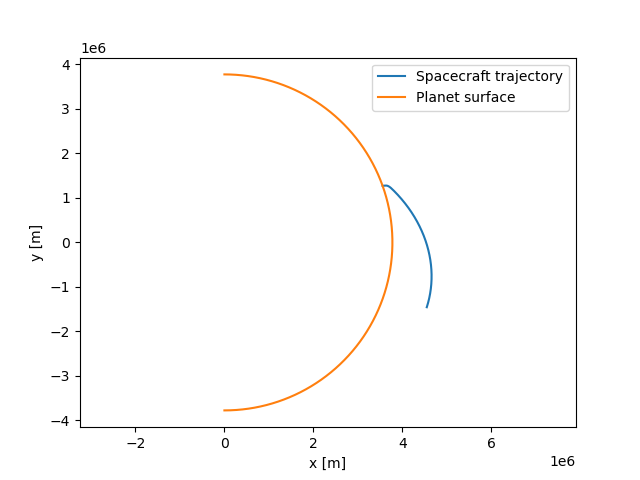
\includegraphics[scale=0.4]{Figures/sim_landing_far}
    \caption{The trajectory of the spacecraft during the simulated landing.}\label{fig:sim_landing_far}
\end{figure}

\begin{figure}[h]
    %% H(Here), h(here approx), t(top of page), b(bottom of page)
    \centering
    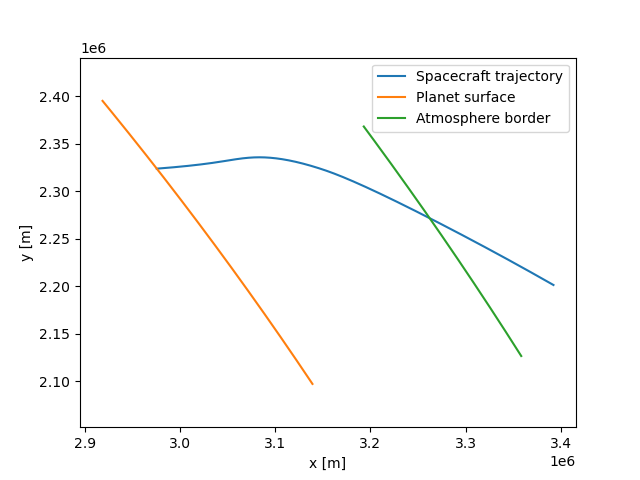
\includegraphics[scale=0.4]{Figures/sim_landing_close}
    \caption{The last part of the trajectory of the spacecraft during the simulated landing from a closer perspective.}\label{fig:sim_landing_close}
\end{figure}

\begin{figure}[h]
    %% H(Here), h(here approx), t(top of page), b(bottom of page)
    \centering
    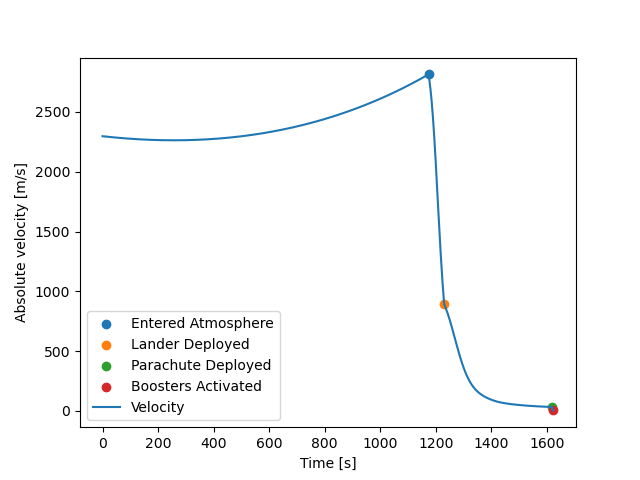
\includegraphics[scale=0.4]{Figures/sim_landing_velocity}
    \caption{The absolute velocity of the spacecraft during the simulated landing.}\label{fig:sim_landing_velocity}
\end{figure}

\begin{figure}[h]
    %% H(Here), h(here approx), t(top of page), b(bottom of page)
    \centering
    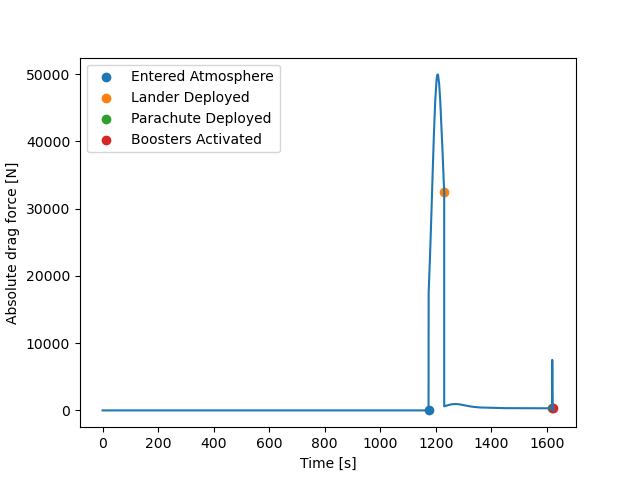
\includegraphics[scale=0.4]{Figures/sim_landing_f_drag}
    \caption{The absolute drag force experienced by the spacecraft during the simulated landing.}\label{fig:sim_landing_f_drag}
\end{figure}



\subsection{Executing the landing}\label{subsec:executing-the-landing}
    After simulating the landing and determining initial values as well as important values like parachute area and lander and parachute deployment height, the actual landing has been executed.
    By using the initial values from~\ref{tab:initial_values}, the spacecraft fell as simulated out of orbit.
    It gained speed until reaching the outer boundary of the atmosphere, where it slowed down substantially due to the atmospheric drag force.\\
    At this point, the spacecraft executes six braking boosts, before reaching a low enough velocity to deploy the lander.
    These can also be seen as spikes in figure~\ref{fig:landing_f_drag} as the spacecraft suddenly accelerates and creates more drag.
    The lander was deployed at an altitude of $1.4 \times 10^5$ meters above the planets surface, and with the same velocity, which the spacecraft had.
    This can also be seen in figure~\ref{fig:landing_velocity}, where the velocity drops to almost 0 before accelerating again due to the gravitational force.\\
    During its fall, the lander reaches its terminal velocity, until the main parachute is deployed at an altitude of 1000 meters above the surface.
    The parachute created a high drag force, which further slowed the lander to a terminal velocity of $6.5$ meters per second.\\
    At an altitude of 200 meters, the landing thrusters were then activated and slowed the lander to it's landing velocity of $2.831$ meters per second.
    The touchdown happened 46 minutes and 3 seconds after initiating the landing sequence and at the coordinates
    \begin{align*}
    \text{x}: 3461.2, \;\text{y}: 1507.6, \;\text{z}: 0
    \end{align*}
    where all values are given in kilometers.
    The trajectory of the spacecraft and lander has been visualized in figures~\ref{fig:landing_far} and~\ref{fig:landing_close}.
    Furthermore, the absolute velocity of the spacecraft and the drag force experienced by the spacecraft during the landing sequence can be seen in respectively figures~\ref{fig:landing_velocity} and~\ref{fig:landing_f_drag}.
    The landing sequence took

\begin{figure}[h]
    %% H(Here), h(here approx), t(top of page), b(bottom of page)
    \centering
    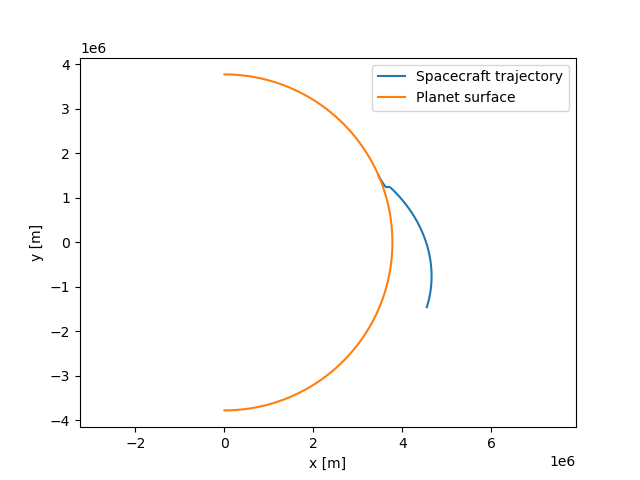
\includegraphics[scale=0.4]{Figures/landing_far}
    \caption{The trajectory of the spacecraft during the landing.}\label{fig:landing_far}
\end{figure}

\begin{figure}[h]
    %% H(Here), h(here approx), t(top of page), b(bottom of page)
    \centering
    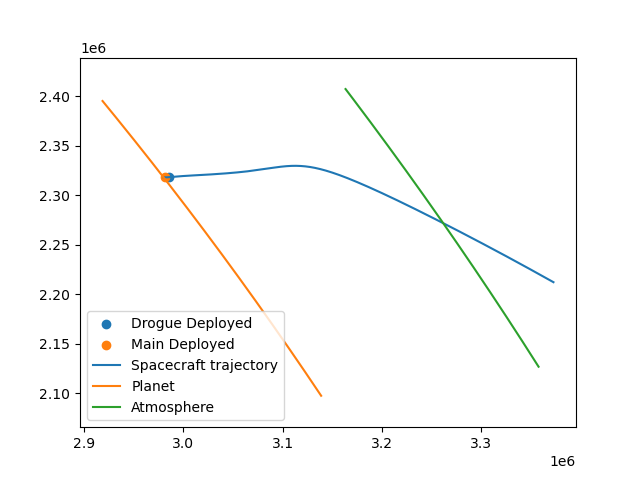
\includegraphics[scale=0.4]{Figures/landing_close}
    \caption{The last part of the trajectory of the spacecraft during the landing from a closer perspective.}\label{fig:landing_close}
\end{figure}

\begin{figure}[h]
    %% H(Here), h(here approx), t(top of page), b(bottom of page)
    \centering
    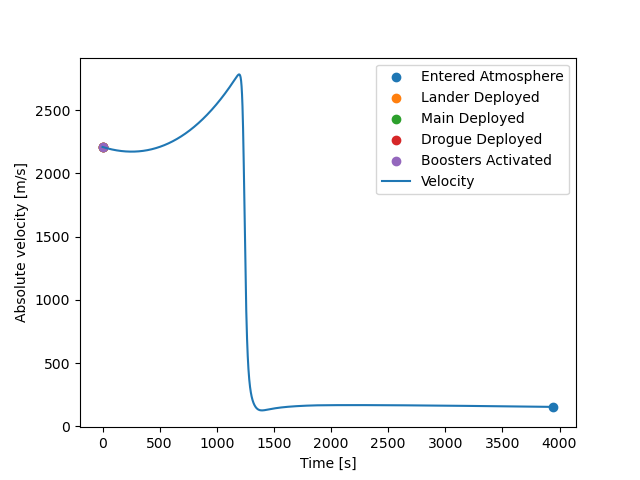
\includegraphics[scale=0.4]{Figures/landing_velocity}
    \caption{The absolute velocity of the spacecraft during the landing.}\label{fig:landing_velocity}
\end{figure}

\begin{figure}[h]
    %% H(Here), h(here approx), t(top of page), b(bottom of page)
    \centering
    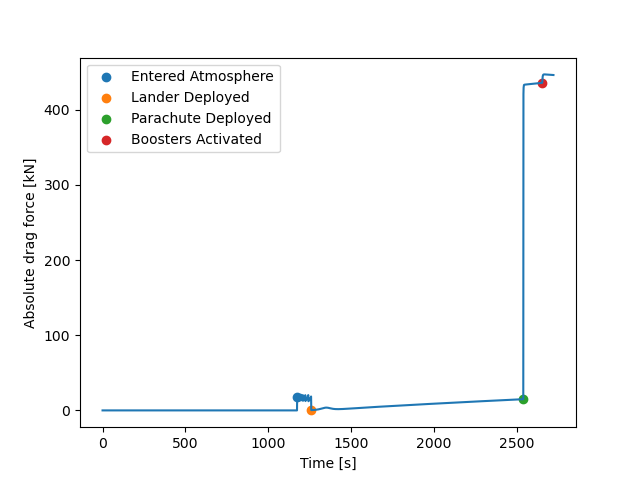
\includegraphics[scale=0.4]{Figures/landing_f_drag}
    \caption{The absolute drag force experienced by the spacecraft during the landing.}\label{fig:landing_f_drag}
\end{figure}


\section{Discussion} \label{sec:discussion}
When comparing the results of the simulation with the results from the actual landing, we can immediately see that there are some differences.
In figures~\ref{fig:sim_landing_far} and~\ref{fig:landing_far} we can see that the trajectory before entering the atmosphere looks identical.
Here, no forces other than gravity are acting, which means there are few things which could lead to a difference.\\

When entering the atmosphere, the trajectory stays almost identical until the lander was deployed.
After launching the lander, however, the trajectory starts to differ.\\
The simulation shows a gradual slow down of tangential speed relative to the planet and a relatively straight path down to the surface.
During the actual landing, the tangential velocity of the lander does not slow down, but rather accelerates.\\
This is an important difference, considering how much more the lander drifts after the lander has been launched relative to the simulation.
A possible explanation for this behaviour are atmospheric winds.
Our simulation only takes into account the rotation of the atmosphere with the planet and assumes that the atmosphere has no angular velocity relative to the planet.\\
In reality, the movement of the atmosphere is much more complex containing winds in all directions.
Especially in the lower part of the atmosphere where the atmosphere is denser, winds can therefore impact the trajectory of the lander significantly.
Both trajectories are therefore possible, considering these atmospheric winds.\\
This could be something to take into account in more detailed simulations, when a more precise landing is required, but as we have chosen a relatively large landing site, this was assumed to not be necessary.\\

The absolute velocity which can be seen in figures~\ref{fig:sim_landing_velocity} and~\ref{fig:landing_velocity}, seems to behave similarly.
The spacecraft accelerates as long as it is outside the atmosphere, and decelerates rapidly once entering the atmosphere.\\
During the actual landing, some braking boosts were necessary to slow the spacecraft down until reaching a low enough velocity to deploy the lander.
In the simulation, the spacecraft was able to slow down enough on its own without exceeding its drag pressure limit of $10^7$ Pascal.\\
However, after the lander was launched, the behaviour of the velocity during the actual landing starts to differ from the simulation.
This is of course connected, but no necessarily due to the difference of the trajectory stated above.\\
In the simulation, the lander gradually slows down further until reaching its terminal velocity and slowing even more after deploying the parachute.
The actual landing actually showed a little increase in speed after the lander was deployed.
This is most likely due to the actual deployment maneuver impacting the velocity of the lander before it could then slow down further.\\
The last part is again relatively similar to the simulation, as the lander decelerates until reaching its terminal velocity and then falling at its terminal velocity until the parachute is deployed.
Compared to the simulation, however, this last section of falling at its terminal velocity is much longer.\\

This correlates clearly to the much longer drift, seen in the actual landing.
As the lander seems to deploy at approximately the same time, the fall of the lander must take significantly longer than in the simulation.
The duration of this part in the actual landing does make much more sense than the simulation, as the lander is deployed at an altitude of $1.4 \times 10^5$ meters above the surface.
It would therefore have to fall with a much higher velocity than the terminal velocity calculated earlier.\\
By looking at the values for the drag force, we can also see that the drag force after the lander is deployed is much higher in the actual landing than in the simulation.
Especially after the deployment of the parachute, we see a large difference, resulting in a much slower terminal velocity and descent of the lander.
This would mean that the simulation is not entirely correct due to human error.
This is a valid source of error even with an experienced team of researchers.\\

Nevertheless, the landing sequence itself was correct, and lead to a successful landing of the spacecraft relatively close to the landing site.
The landing coordinates were off by $4.08 \times 10^{-3}$ degrees of longitude
This means, the landing happened 269 meters east of the landing site.
Such a difference in latitude is almost negligible for a landing maneuver with so many variables, and could most likely be explained due to wind or inaccuracies of some maneuvers, which means we were able to land successfully at our landing site.


\section{Conclusion} \label{sec:conclusion}
To reach our destination, we now had to actually land the lander on the surface of the planet.
This required the creation of a simulation beforehand, as such a landing includes many variables and forces such as gravity, drag, winds and the motion of the planet itself.
Our team of researchers created a simulation, which was able to simulate the trajectory of the spacecraft from the orbit until the landing, including events such as lander and parachute deployment and activation of the landing thrusters.\\

This simulation was then used to determine initial values for the position and velocity of the spacecraft when we initiate the landing, as well as altitudes for the deployment of the lander and parachute.\\

By using the values from the simulation, the spacecraft was able to execute the landing procedure and follow a very similar trajectory as simulated.
After launching the lander however, the trajectory started to differentiate from the simulated trajectory, which meant the lander drifted further than anticipated.
When looking into this deviance, we found that this is due to a difference in drag force after the lander was launched, and especially after the parachute was deployed.\\

However, the landing procedure itself was executed as planned, which resulted in a landing at the coordinates $\text{x:} \;3461.2, \;\text{y:} \;1507.6, \;\text{z:} \;0.0$ (all given in kilometers) at a velocity of $2.831$ meters per second.
This is 269 meters east of the planned landing site, and below the maximum landing velocity of 3 meters per second.
We were therefore successfully able to land on the island we picked as a landing site in% ~\parencite[][]{part6}. TODO: Delete Comment


\section{Appendix} \label{sec:appendix}
\subsection{Calculating the parachute area}\label{subsec:calculating-the-parachute-area}
    The required parachute area for a given terminal velocity can be found by using newtons second law and combining the formulas for gravitational acceleration~\eqref{f_g} and drag force~\eqref{f_d}.
    \begin{align}
        F_G &= -G\;\frac{M m}{R^2} \label{f_g}\\
        F_D &= \frac{1}{2}\rho \,C_D A v^2 \label{f_d}
    \end{align}
    Where G is the universal gravitational constant, M is the mass of the planet, m is the mass of the lander, $\rho$ is the density of the atmosphere, $C_D$ is the drag coefficient, A is the combined area of attack of the lander and parachute, and v is the velocity.
    At the terminal velocity, the acceleration is 0.
    This means that $F_G = F_D$.\\
    By rearranging the formulae we get
    \begin{align*}
        A = \frac{2 G M m}{\rho C_D R^2 v^2}
    \end{align*}
    If we want to calculate the area needed for a safe landing, we will have to insert the mass of the planet and spacecraft, the density of the atmosphere at the surface, the radius of the planet and the maximum velocity of 3 meters per second.


\subsection{Parachute area with boosters}\label{subsec:parachute-area-with-boosters}
    When including landing boosters, we can decrease the parachute area.
    The exact amount depends on the thrust of the landing boosters $F_T$ and can again be calculated using newtons second law and equations~\eqref{f_g} and~\ref{f_d}.
    Now we have the equation
    \begin{align}
        F_G + F_D + F_T = 0\\
        F_T = - F_G - F_D \label{eq1}
    \end{align}
Furthermore we know that at the terminal velocity for our parachute size $v_t$,
\begin{align}
    F_G = -\frac{1}{2}\rho \,C_D A v_t^2 \label{f_g1}
\end{align}

We also know that the drag force from the parachute at the landing velocity $v_{land}$ while using the landing boosters is
\begin{align}
    F_D = \frac{1}{2}\rho \,C_D A v_{land}^2 \label{f_d1}
\end{align}

By inserting formulae~\ref{f_g1} and~\ref{f_d1} into~\ref{eq1}, we get find that
\begin{align}
    F_T = \frac{1}{2}\rho \,C_D A \left(v_t^2 - v_{land}^2 \right)
\end{align}

This can be rearranged to find the required area of the parachute.
\begin{align}
    A = \frac{2}{\rho \,C_D v_{land}^2}\left( G\,\frac{M m}{R^2} - F_D \right)
\end{align}
By inserting known values for $v_{land}$ and $F_T$ we can find the parachute area while using boosters for our lander.


\newpage
% \printbibliography TODO: Remove Comment

\end{document}

